\section{Variance and standard deviation of $\xt$ and $\wt$}
\label{sec:variance}

To describe the variance of a random variable, we use the standard formula
\begin{equation*}
\text{Var}(\xt) = \mean{\xt^2} - \mean{\xt}^2,
\end{equation*}
and we apply it to $\xt$ and $\wt$ to quantify the variability of intracellular
and extracellular particle counts as functions of time. In each case, we first
require a formula for the expected value of the count squared: $\mean{\xt^2}$
and $\mean{\wt^2}$.

\subsection{Variance of $\xt$}

\subsubsection{Formula for $\mean{\xt^2}$ $(=K(t))$}

A formula for $K(t) = \mean{\xt^2}$ is derived in the following way. Take the
time derivative of the two equations
$$\text{(\ref{ddIJ}):}\quad {\rm d}I/{\rm d}t = -\delta J,\qquad
\text{(\ref{ddII}):}\quad {\rm d}I/{\rm d}t = \mu - (\lambda + \mu + \delta) I + \lambda I^2.$$
From the first,
\begin{equation}
\label{Kderev1}
\ddt{J} = -\frac{1}{\delta}\frac{\dd^2 I}{\dd t^2},
\end{equation}
while differentiating the second gives
$$\frac{\dd^2 I}{\dd t^2} = -(\lambda + \mu + \delta) \ddt{I} + 2\lambda I \ddt{I},$$
which, with ${\rm d}I/{\rm d}t = -\delta J$, becomes
\begin{equation}
\label{Kderev2}
\frac{\dd^2 I}{\dd t^2} = (\lambda + \mu + \delta)\lambda J- 2\lambda \delta I J.
\end{equation}
Comparing (\ref{Kderev2}) with (\ref{Kderev1}),
$$\ddt{J} = -(\lambda + \mu + \delta) J + 2\lambda I J;$$
then, equating this with (\ref{ddJ2}),
$$(\lambda - \mu) J - \delta K = -(\lambda + \mu + \delta) J + 2\lambda I J.$$
Rearranging for $K(t)$,
\begin{equation}
\label{Kt1}
K(t) = \frac{2\lambda}{\delta}\lrb{1+\frac{\delta}{2\lambda} - I}J
= \Bigl[1+\frac{2\lambda}{\delta}(1-I)\Bigr]J
= \frac{2\lambda}{\delta}(\kappa - I)J,
\end{equation}
with
$$\kappa = 1+\frac{\delta}{2\lambda}.$$

\begin{theorem}
\label{thm:K}
The second moment of the process state is
\begin{equation}
\label{eq:Kclosedform}
K(t)=\Bigl[1+\frac{2\lambda}{\delta}(1-I)\Bigr]J
=\frac{2\lambda}{\delta}(\kappa-I)J,
\end{equation}
and, written as a function of $I$ alone using
$J=-\delta^{-1}I'=-\frac{\lambda}{\delta}(I-a)(I-b)$,
\begin{equation}
\label{eq:KI}
K(I) = \frac{2\lambda^2}{\delta^2}(I-\kappa)(I-a)(I-b).
\end{equation}
\end{theorem}

The factored form \eqref{eq:KI} shows at a glance that $K$ shares the
vanishing of $J$ at both absorbing limits $I\to a$ and $I\to b$, as it must:
a fixed process has no second moment to speak of either.

\subsubsection{One standard deviation from the mean, $J(t)$}

With the expectation of $\xt^2$ in the form (\ref{Kt1}), we can write down the
variance of $\xt$ using $\text{Var}(\xt) = \mean{\xt^2} - \mean{\xt}^2$:
\begin{align*}
\text{Var}(\xt) &= K(t) - {J(t)}^2\\
&= \frac{2\lambda}{\delta}\lrb{\kappa - I}J - J^2,
\end{align*}
and the standard deviation is then
\begin{equation*}
\text{Std}(\xt) = \sqrt{\frac{2\lambda}{\delta}\lrb{\kappa- I}J - J^2}.
\end{equation*}

\subsection{Variance of $\wt$}

We can likewise compute the variance of $\wt$ using
$\text{Var}(\wt) = \mean{\wt^2} - \mean{\wt}^2$. To begin, we must find a
formula for $\mean{\wt^2}$.

\subsubsection{Formula for $\mean{\wt^2}$}

Accounting for changes to $\wt^2$ over an infinitesimal time $\delt$,
$$\mean{\ww_{t+\delt}^2} = \mean{\wt^2} + \mean{\ww_{t+\delt}^2 - \wt^2},$$
we can derive the equation
\begin{equation}
\label{meanYt2}
\ddt{\mean{\wt^2}} = \delta \mean{\xt^3}:
\end{equation}
when rupture occurs from state $n$, at rate $\delta n$, the released count
jumps from $0$ to $n$, so $\wt^2$ gains $n^2$, and the rate-times-jump
contribution is $\delta n^3$. This might seem like a dead end, since we have
yet to produce a description of $\mean{\xt^3}$. As it happens, the problem can
be sidestepped by thinking about the rate of change of $K(t)=\mean{\xt^2}$:
\begin{equation}
\label{meanysq1}
\mean{\xx_{t+\delt}^2} = \mean{\xt^2} + \mean{\xx_{t+\delt}^2 - \xt^2}.
\end{equation}
Because of the quadratic, changes in $\xt^2$ require special attention
(\Tabref{tab:xsqchanges}).
\begin{table}[ht]
\centering
\renewcommand{\arraystretch}{1.5}
\setlength{\tabcolsep}{17pt}
\begin{tabular}{|>{\centering\arraybackslash}m{3cm}|>{\centering\arraybackslash}m{2cm}|>{\centering\arraybackslash}m{5cm}|}
\hline
Probability of occurrence& Change in $\xt$ & Change in $\xt^2$\\
\hline
\hline
$\lambda \xt\delt$& 1 & $(\xt + 1)^2 - \xt^2 = 2\xt + 1$ \\
\hline
$\mu \xt\delt$ &-1 & $(\xt - 1)^2 - \xt^2 = -2\xt + 1$\\
\hline
$\delta \xt\delt$ & $-\xt$& $(\xt - \xt)^2 - \xt^2 = -\xt^2$ \\
\hline
\end{tabular}
\caption{The three event types and their contributions to $\xt^2$.}
\label{tab:xsqchanges}
\end{table}

\noindent
From the possibilities in the table,
\begin{align*}
\mean{\xx_{t+\delt}^2 - \xt^2}
&=\mean{\lambda \xt\delt\cdot(2\xt+1) + \mu \xt\delt\cdot(-2\xt+1) + \delta \xt\delt\cdot(-\xt^2)}\\
&=\bigg[ 2(\lambda-\mu)\mean{\xt^2} + (\lambda+\mu)\mean{\xt} - \delta\mean{\xt^3} \bigg]\delt.
\end{align*}
Taking this with (\ref{meanysq1}), the following equation is obtained in the
$\delt\to0$ limit:
\begin{equation}
\label{ddK2}
\ddt{K} =2(\lambda-\mu)K+ (\lambda + \mu)J- \delta\mean{\xt^3}.
\end{equation}
Equations (\ref{meanYt2}) and (\ref{ddK2}) together eliminate the third moment:
\begin{equation}
\label{dWsqOde}
\ddt{\mean{\wt^2}} = 2(\lambda-\mu)K + (\lambda+\mu)J - \ddt{K}.
\end{equation}
Integrating from $0$ to $t$, and using $V'=\delta K$ (\ref{ddV}) and
$I'=-\delta J$ (\ref{ddIJ}) to evaluate the two integrals,
\begin{align*}
\mean{\wt^2}
&= 2(\lambda-\mu)\int_0^t K\,\dd s + (\lambda+\mu)\int_0^t J\,\dd s - K(t) + K(0)\\
&= \frac{2(\lambda-\mu)}{\delta}V(t) + \frac{\lambda+\mu}{\delta}\bigl(1-I(t)\bigr) - K(t) + K(0).
\end{align*}
The integration constant here is $K(0)=\mean{\xx_0^2}=1$, since the process
begins with a single unit, and $\mean{\ww_0^2}=0$ contributes nothing on the
left. Therefore:

\begin{theorem}
\label{thm:Wsq}
The second moment of the released count is
\begin{equation}
\label{eq:Wsq}
\mean{\wt^2} = \frac{2(\lambda-\mu)}{\delta} V -\frac{\lambda+\mu}{\delta}I -K +\frac{\lambda+\mu}{\delta}+1.
\end{equation}
\end{theorem}

As a check, when $\mu=0$ we have $b=0$, so every realisation ruptures,
$I(\infty)=0$ and $K(\infty)=0$, while $V(\infty)=1+\lambda/\delta$; the
formula gives
$$\mean{\wt^2}\Big|_{t\to\infty} = \frac{2\lambda}{\delta}\Bigl(1+\frac{\lambda}{\delta}\Bigr) + \frac{\lambda}{\delta} + 1 = \frac{2\lambda^2}{\delta^2}+\frac{3\lambda}{\delta}+1.$$
This is exactly the second moment of the geometric burst-size law
$P_k=(\delta/\lambda)a^{-k}$ with $a=(\lambda+\delta)/\lambda$ --- a geometric
distribution on $\{1,2,\ldots\}$ with success probability
$\delta/(\lambda+\delta)$, whose second moment is $(2-s)/s^2$ for $s=\delta/(\lambda+\delta)$.
The burst-size law itself is derived in Chapter~4a; for now the agreement
confirms \eqref{eq:Wsq}.

\subsubsection{One standard deviation from the mean, $V(t)$}

Using (\ref{eq:Wsq}), it is possible to write down a formula for the variance
of $\wt$:
\begin{equation}
\label{VarY}
\text{Var}(\wt) = \frac{2(\lambda-\mu)}{\delta} V -\frac{\lambda+\mu}{\delta}I -K +\frac{\lambda+\mu}{\delta}+1 - V^2.
\end{equation}

\begin{figure}[H]
\centering
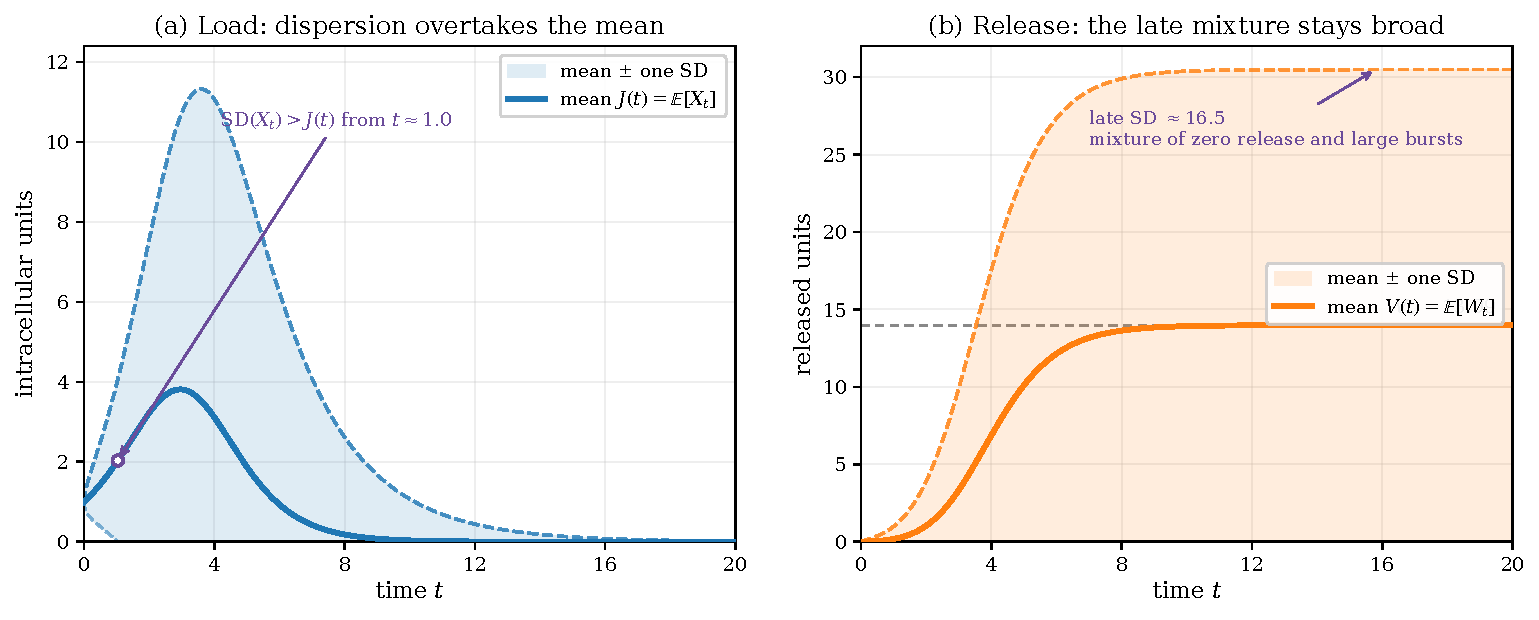
\includegraphics[width=0.98\textwidth]{figures/N3_1_mean_sd_XW.pdf}
\caption{Mean and one-standard-deviation envelopes for the intracellular load
$\xt$ (a) and released count $\wt$ (b), for $\lambda=1$, $\mu=0.2$, and
$\delta=0.05$. The lower envelope is clipped at zero, the support boundary for
both counts. Load dispersion overtakes $J(t)$ early in the productive window,
while the late spread in $\wt$ records the mixture of never-rupturing paths and
large releases. Means alone therefore conceal substantial pathwise
uncertainty.}
\label{fig:N3_1}
\end{figure}
